\hypertarget{interfaceDataValue}{
\section{Data\-Value  Interface Reference}
\label{interfaceDataValue}\index{DataValue@{Data\-Value}}
}
Inheritance diagram for Data\-Value:\begin{figure}[H]
\begin{center}
\leavevmode
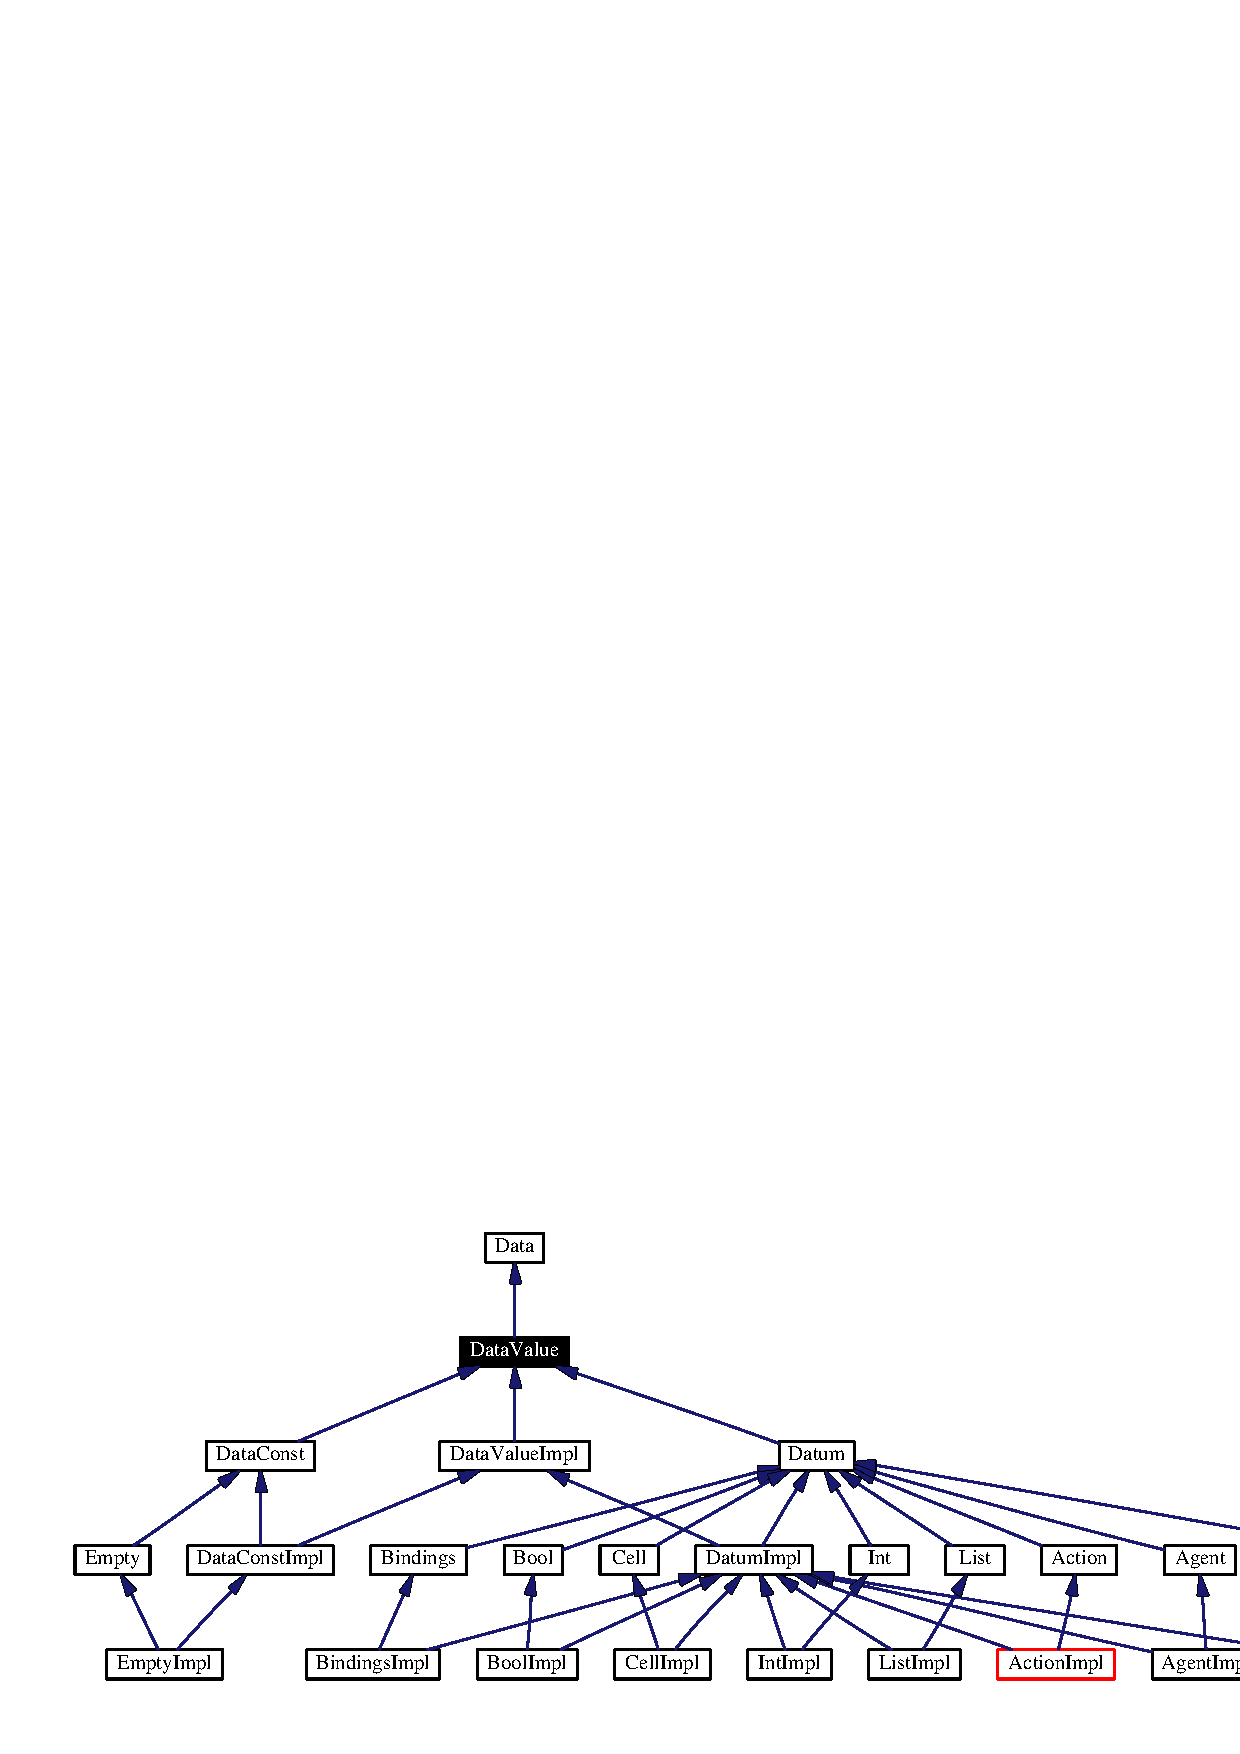
\includegraphics[width=400pt]{interfaceDataValue__inherit__graph}
\end{center}
\end{figure}
Collaboration diagram for Data\-Value:\begin{figure}[H]
\begin{center}
\leavevmode
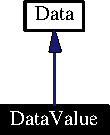
\includegraphics[width=44pt]{interfaceDataValue__coll__graph}
\end{center}
\end{figure}
\subsection*{Public Methods}
\begin{CompactItemize}
\item 
\hyperlink{interfaceEmpty}{Empty} \hyperlink{interfaceDataValue_a0}{equals} (\hyperlink{interfaceData}{Data} data) throws \hyperlink{classExceptional}{Exceptional}
\end{CompactItemize}


\subsection{Member Function Documentation}
\hypertarget{interfaceDataValue_a0}{
\index{DataValue@{Data\-Value}!equals@{equals}}
\index{equals@{equals}!DataValue@{Data\-Value}}
\subsubsection[equals]{\setlength{\rightskip}{0pt plus 5cm}\hyperlink{interfaceEmpty}{Empty} Data\-Value::equals (\hyperlink{interfaceData}{Data} {\em data})}}
\label{interfaceDataValue_a0}




Reimplemented in \hyperlink{classActionImpl_a21}{Action\-Impl}, \hyperlink{classBoolImpl_a2}{Bool\-Impl}, \hyperlink{classDataValueImpl_a5}{Data\-Value\-Impl}, \hyperlink{classIntImpl_a9}{Int\-Impl}, \hyperlink{classListImpl_a5}{List\-Impl}, and \hyperlink{classTextImpl_a1}{Text\-Impl}.

Referenced by List\-Impl::equals().



The documentation for this interface was generated from the following file:\begin{CompactItemize}
\item 
\hyperlink{DataValue_8java-source}{Data\-Value.java}\end{CompactItemize}
